\documentclass{article}
\title{Homework4.1}
\author{Blue}
\date{20230224}
\usepackage{geometry}
\geometry{a4paper,scale=0.8}
\usepackage{graphicx}
\usepackage{float}
\usepackage{indentfirst}
\usepackage[namelimits]{amsmath} %数学公式
\usepackage{amssymb}             %数学公式
\usepackage{color}
\usepackage{longtable}
\usepackage{listings}
\usepackage{float}
\lstset{
language=Matlab,
numbers=left,
keywordstyle=\color{blue},
numberstyle=\tiny,
breaklines=true,
extendedchars=flase
}
\begin{document}
\maketitle
\section{Results}
\subsection{Movie}
The movie code is attached to the end of the document.
\subsection{Track the position}
We keep track of the position of the 10,100,1000 particles and plot their positions. The Figure \ref{figure1} shows the distribution of their final position. The purple dot is the position of one particles, while the yellow dots are the positions of the 10 points. The green dots shows the position of 100 particles, while the red dots are the positions of the 1000 particles' random walk.
\begin{figure}[H]
\centering
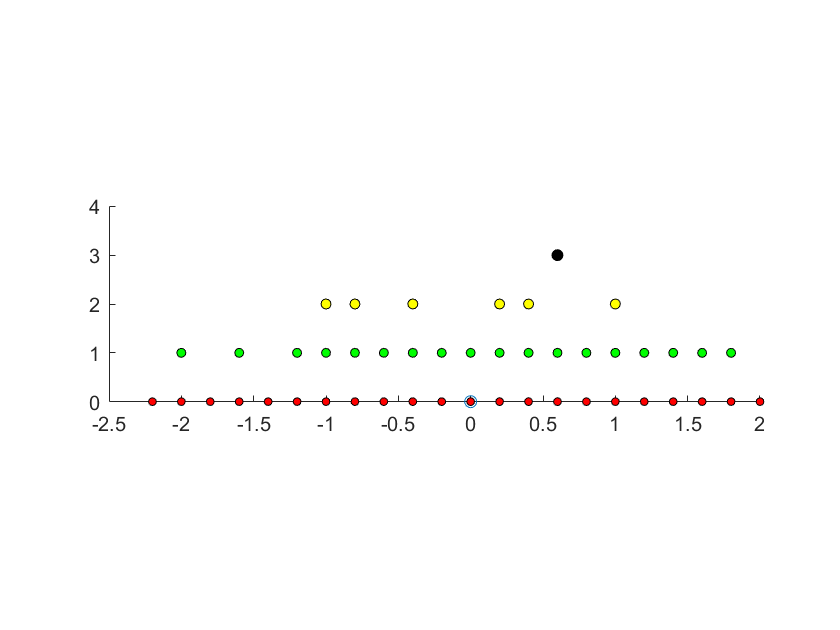
\includegraphics[width=4.00in,height=3.00in]{Distribution.png} 
\caption{Distribution of the points}
\label{figure1}
\end{figure}
To exam it more thoroughly, I plot the histogram of their position and gets the following results. The histogram of the distribution of the particles' positions looks like a normal distribution.
\clearpage
\begin{figure}[htbp]
    \centering
    \begin{minipage}{0.45\linewidth}
        \centering
        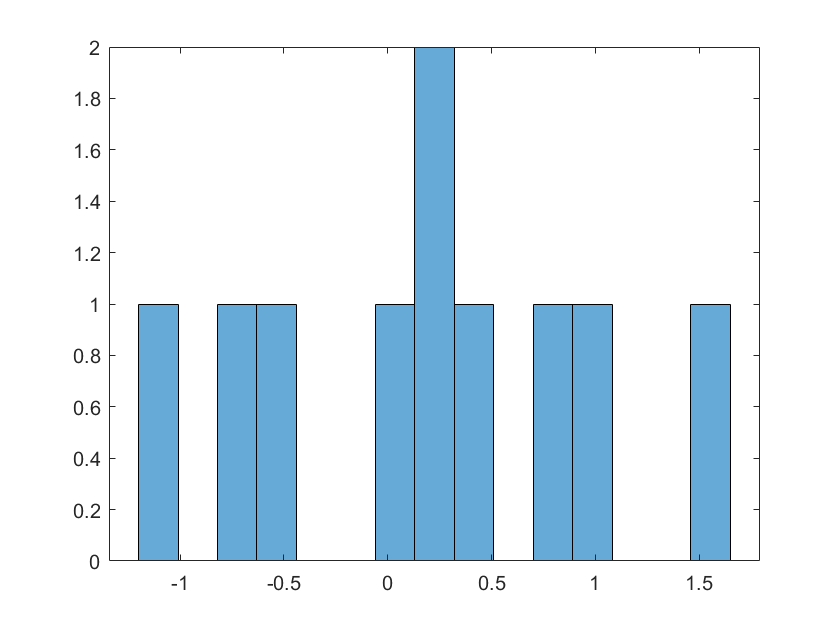
\includegraphics[width=0.8\linewidth]{walk10.png}
        \caption{The histogram of 10 points final positions}
    \end{minipage}
    \hfill
    \begin{minipage}{0.45\linewidth}
        \centering
        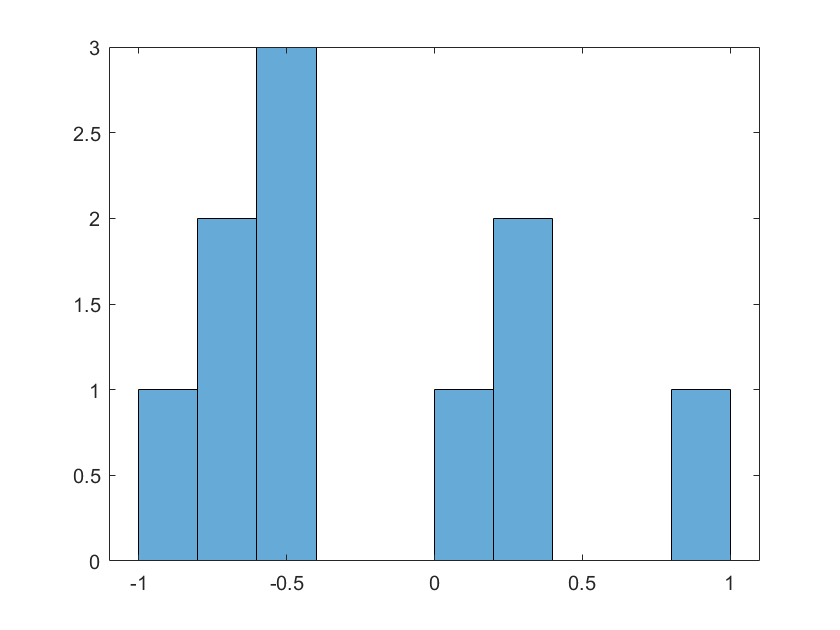
\includegraphics[width=0.8\linewidth]{walk101.png}
        \caption{The histogram of 10 points final positions}
    \end{minipage}
\end{figure}

\begin{figure}[htbp]
    \centering
    \begin{minipage}{0.45\linewidth}
        \centering
        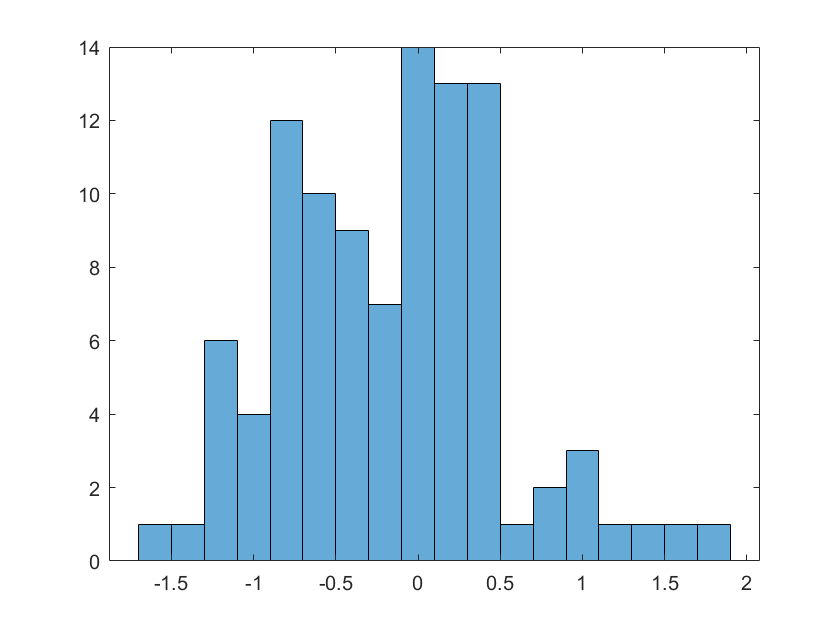
\includegraphics[width=\linewidth]{walk100.png}
        \caption{The histogram of 100 points final positions}
    \end{minipage}
    \hfill
    \begin{minipage}{0.45\linewidth}
        \centering
        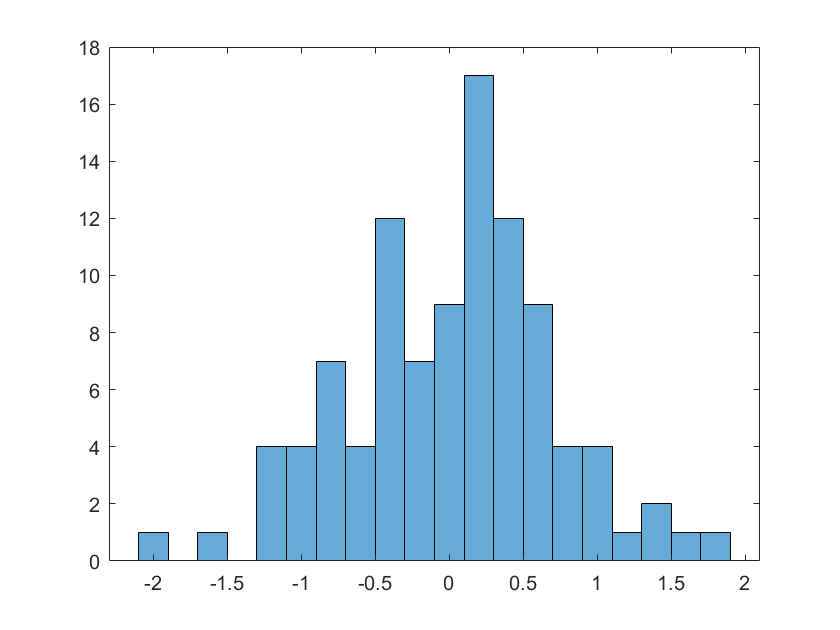
\includegraphics[width=\linewidth]{walk1001.png}
        \caption{The histogram of 100 points final positions}
    \end{minipage}
\end{figure}

\begin{figure}[H]
    \centering
    \begin{minipage}{0.45\linewidth}
        \centering
        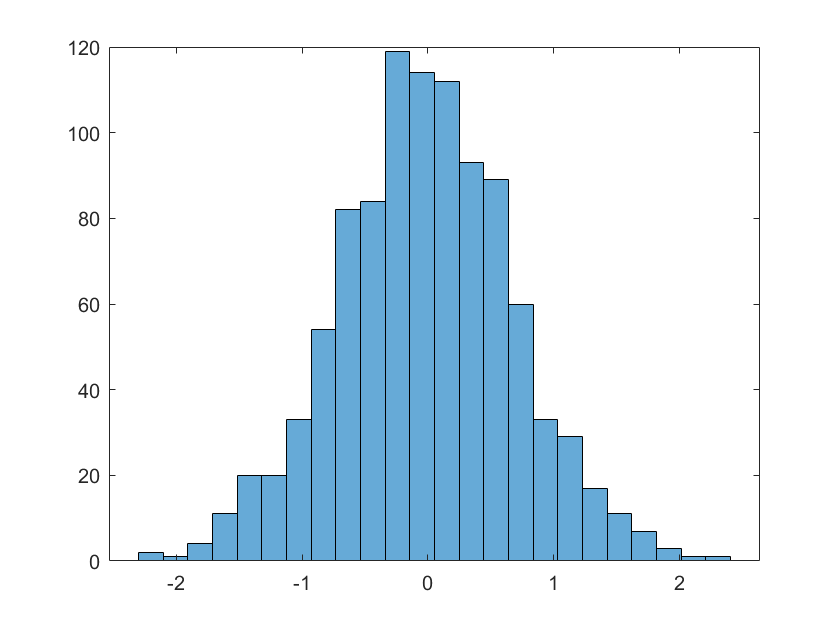
\includegraphics[width=\linewidth]{walk1000.png}
        \caption{The histogram of 1000 points final positions}
    \end{minipage}
    \hfill
    \begin{minipage}{0.45\linewidth}
        \centering
        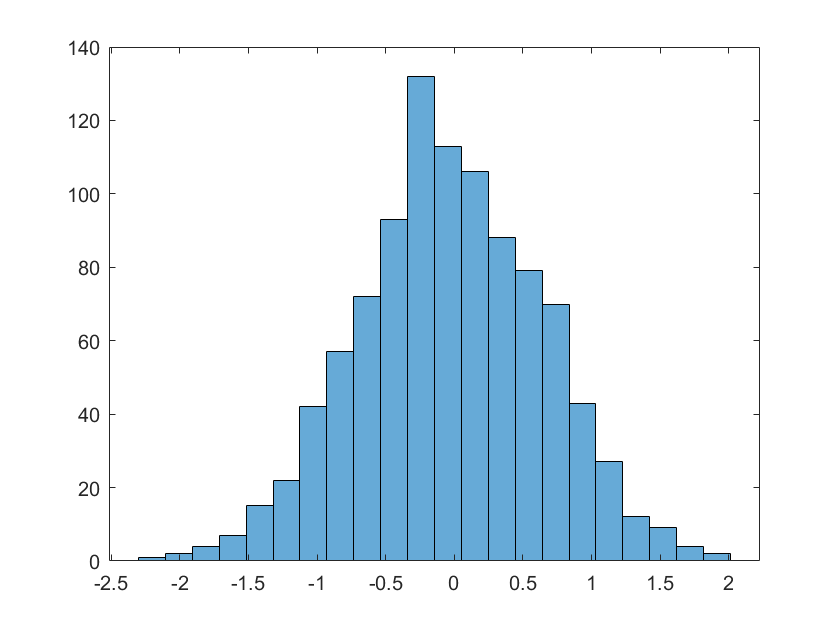
\includegraphics[width=\linewidth]{walk10001.png}
        \caption{The histogram of 1000 points final positions}
    \end{minipage}
\end{figure}
\clearpage




\section{code}
\subsection{Random walk movie}
\begin{lstlisting}
nSteps = 50;
startPos = 0;
stepSize = 0.1;
steps = stepSize * (2 * randi([0, 1], nSteps, 1) - 1);
walk = cumsum(steps) + startPos;
plot(walk);
k=5;
vidobj = VideoWriter('test.mp4','mpeg-4');
open(vidobj);
for i=1:nSteps*k-1
    scatter(walk(floor(i/k)+1),0,50,'ok','markerfacecolor','r')
    xlim([min(walk) max(walk)])
    ylim([0 0.5])
    pbaspect([100 30 1])
    title('Random walk')
    currFrame = getframe(gcf);
    writeVideo(vidobj,currFrame);
end
close(vidobj);
\end{lstlisting}


\subsection{Track the position}
\begin{lstlisting}
walk1=walkf(50,1,0.1);
walk2=walkf(50,10,0.1);
walk3=walkf(50,100,0.1);
walk4=walkf(50,1000,0.1);
figure(1)
scatter(0,0);hold on
spwalk(walk4,'r',15,1);
spwalk(walk3,'g',20,2);
spwalk(walk2,'y',25,3);
spwalk(walk1,'k',30,4);
ylim([0,4])
pbaspect([100 30 1])
hold off
figure(2)
bins3=floor((max(walk3)-min(walk3))/0.2+1);
histogram(walk3,bins3);
figure(3)
bins4=floor((max(walk4)-min(walk4))/0.2+1);
histogram(walk4,bins4);
figure(4)
bins2=floor((max(walk2)-min(walk2))/0.2+1);
histogram(walk2,bins2);


function walks=walkf(nSteps,size,stepSize)
walks=zeros(size,1);
for i=1:size
    steps = stepSize * (2 * randi([0, 1], nSteps, 1) - 1);
    walk = cumsum(steps);
    walks(i)=walk(nSteps);
end
end

function spwalk(walk,col,siz,j)
[m,n]=size(walk);
for i=1:m
    scatter(walk(i),j-1,siz,'ok','markerfacecolor',col);
end
end
\end{lstlisting}





\end{document}